% Options for packages loaded elsewhere
\PassOptionsToPackage{unicode}{hyperref}
\PassOptionsToPackage{hyphens}{url}
%
\documentclass[
  ignorenonframetext,
]{beamer}
\usepackage{pgfpages}
\setbeamertemplate{caption}[numbered]
\setbeamertemplate{caption label separator}{: }
\setbeamercolor{caption name}{fg=normal text.fg}
\beamertemplatenavigationsymbolsempty
% Prevent slide breaks in the middle of a paragraph
\widowpenalties 1 10000
\raggedbottom
\setbeamertemplate{part page}{
  \centering
  \begin{beamercolorbox}[sep=16pt,center]{part title}
    \usebeamerfont{part title}\insertpart\par
  \end{beamercolorbox}
}
\setbeamertemplate{section page}{
  \centering
  \begin{beamercolorbox}[sep=12pt,center]{part title}
    \usebeamerfont{section title}\insertsection\par
  \end{beamercolorbox}
}
\setbeamertemplate{subsection page}{
  \centering
  \begin{beamercolorbox}[sep=8pt,center]{part title}
    \usebeamerfont{subsection title}\insertsubsection\par
  \end{beamercolorbox}
}
\AtBeginPart{
  \frame{\partpage}
}
\AtBeginSection{
  \ifbibliography
  \else
    \frame{\sectionpage}
  \fi
}
\AtBeginSubsection{
  \frame{\subsectionpage}
}
\usepackage{lmodern}
\usepackage{amssymb,amsmath}
\usepackage{ifxetex,ifluatex}
\ifnum 0\ifxetex 1\fi\ifluatex 1\fi=0 % if pdftex
  \usepackage[T1]{fontenc}
  \usepackage[utf8]{inputenc}
  \usepackage{textcomp} % provide euro and other symbols
\else % if luatex or xetex
  \usepackage{unicode-math}
  \defaultfontfeatures{Scale=MatchLowercase}
  \defaultfontfeatures[\rmfamily]{Ligatures=TeX,Scale=1}
\fi
% Use upquote if available, for straight quotes in verbatim environments
\IfFileExists{upquote.sty}{\usepackage{upquote}}{}
\IfFileExists{microtype.sty}{% use microtype if available
  \usepackage[]{microtype}
  \UseMicrotypeSet[protrusion]{basicmath} % disable protrusion for tt fonts
}{}
\makeatletter
\@ifundefined{KOMAClassName}{% if non-KOMA class
  \IfFileExists{parskip.sty}{%
    \usepackage{parskip}
  }{% else
    \setlength{\parindent}{0pt}
    \setlength{\parskip}{6pt plus 2pt minus 1pt}}
}{% if KOMA class
  \KOMAoptions{parskip=half}}
\makeatother
\usepackage{xcolor}
\IfFileExists{xurl.sty}{\usepackage{xurl}}{} % add URL line breaks if available
\IfFileExists{bookmark.sty}{\usepackage{bookmark}}{\usepackage{hyperref}}
\hypersetup{
  pdftitle={Data I/O, Part 1},
  pdfauthor={Data Wrangling in R},
  hidelinks,
  pdfcreator={LaTeX via pandoc}}
\urlstyle{same} % disable monospaced font for URLs
\newif\ifbibliography
\usepackage{color}
\usepackage{fancyvrb}
\newcommand{\VerbBar}{|}
\newcommand{\VERB}{\Verb[commandchars=\\\{\}]}
\DefineVerbatimEnvironment{Highlighting}{Verbatim}{commandchars=\\\{\}}
% Add ',fontsize=\small' for more characters per line
\usepackage{framed}
\definecolor{shadecolor}{RGB}{248,248,248}
\newenvironment{Shaded}{\begin{snugshade}}{\end{snugshade}}
\newcommand{\AlertTok}[1]{\textcolor[rgb]{0.94,0.16,0.16}{#1}}
\newcommand{\AnnotationTok}[1]{\textcolor[rgb]{0.56,0.35,0.01}{\textbf{\textit{#1}}}}
\newcommand{\AttributeTok}[1]{\textcolor[rgb]{0.77,0.63,0.00}{#1}}
\newcommand{\BaseNTok}[1]{\textcolor[rgb]{0.00,0.00,0.81}{#1}}
\newcommand{\BuiltInTok}[1]{#1}
\newcommand{\CharTok}[1]{\textcolor[rgb]{0.31,0.60,0.02}{#1}}
\newcommand{\CommentTok}[1]{\textcolor[rgb]{0.56,0.35,0.01}{\textit{#1}}}
\newcommand{\CommentVarTok}[1]{\textcolor[rgb]{0.56,0.35,0.01}{\textbf{\textit{#1}}}}
\newcommand{\ConstantTok}[1]{\textcolor[rgb]{0.00,0.00,0.00}{#1}}
\newcommand{\ControlFlowTok}[1]{\textcolor[rgb]{0.13,0.29,0.53}{\textbf{#1}}}
\newcommand{\DataTypeTok}[1]{\textcolor[rgb]{0.13,0.29,0.53}{#1}}
\newcommand{\DecValTok}[1]{\textcolor[rgb]{0.00,0.00,0.81}{#1}}
\newcommand{\DocumentationTok}[1]{\textcolor[rgb]{0.56,0.35,0.01}{\textbf{\textit{#1}}}}
\newcommand{\ErrorTok}[1]{\textcolor[rgb]{0.64,0.00,0.00}{\textbf{#1}}}
\newcommand{\ExtensionTok}[1]{#1}
\newcommand{\FloatTok}[1]{\textcolor[rgb]{0.00,0.00,0.81}{#1}}
\newcommand{\FunctionTok}[1]{\textcolor[rgb]{0.00,0.00,0.00}{#1}}
\newcommand{\ImportTok}[1]{#1}
\newcommand{\InformationTok}[1]{\textcolor[rgb]{0.56,0.35,0.01}{\textbf{\textit{#1}}}}
\newcommand{\KeywordTok}[1]{\textcolor[rgb]{0.13,0.29,0.53}{\textbf{#1}}}
\newcommand{\NormalTok}[1]{#1}
\newcommand{\OperatorTok}[1]{\textcolor[rgb]{0.81,0.36,0.00}{\textbf{#1}}}
\newcommand{\OtherTok}[1]{\textcolor[rgb]{0.56,0.35,0.01}{#1}}
\newcommand{\PreprocessorTok}[1]{\textcolor[rgb]{0.56,0.35,0.01}{\textit{#1}}}
\newcommand{\RegionMarkerTok}[1]{#1}
\newcommand{\SpecialCharTok}[1]{\textcolor[rgb]{0.00,0.00,0.00}{#1}}
\newcommand{\SpecialStringTok}[1]{\textcolor[rgb]{0.31,0.60,0.02}{#1}}
\newcommand{\StringTok}[1]{\textcolor[rgb]{0.31,0.60,0.02}{#1}}
\newcommand{\VariableTok}[1]{\textcolor[rgb]{0.00,0.00,0.00}{#1}}
\newcommand{\VerbatimStringTok}[1]{\textcolor[rgb]{0.31,0.60,0.02}{#1}}
\newcommand{\WarningTok}[1]{\textcolor[rgb]{0.56,0.35,0.01}{\textbf{\textit{#1}}}}
\usepackage{graphicx,grffile}
\makeatletter
\def\maxwidth{\ifdim\Gin@nat@width>\linewidth\linewidth\else\Gin@nat@width\fi}
\def\maxheight{\ifdim\Gin@nat@height>\textheight\textheight\else\Gin@nat@height\fi}
\makeatother
% Scale images if necessary, so that they will not overflow the page
% margins by default, and it is still possible to overwrite the defaults
% using explicit options in \includegraphics[width, height, ...]{}
\setkeys{Gin}{width=\maxwidth,height=\maxheight,keepaspectratio}
% Set default figure placement to htbp
\makeatletter
\def\fps@figure{htbp}
\makeatother
\setlength{\emergencystretch}{3em} % prevent overfull lines
\providecommand{\tightlist}{%
  \setlength{\itemsep}{0pt}\setlength{\parskip}{0pt}}
\setcounter{secnumdepth}{-\maxdimen} % remove section numbering

\title{Data I/O, Part 1}
\author{Data Wrangling in R}
\date{}

\begin{document}
\frame{\titlepage}

\begin{frame}[fragile]{Explaining output on slides}
\protect\hypertarget{explaining-output-on-slides}{}

In slides, a command (we'll also call them code or a code chunk) will
look like this

\begin{Shaded}
\begin{Highlighting}[]
\KeywordTok{print}\NormalTok{(}\StringTok{"I'm code"}\NormalTok{)}
\end{Highlighting}
\end{Shaded}

\begin{verbatim}
[1] "I'm code"
\end{verbatim}

And then directly after it, will be the output of the code.\\
So \texttt{print("I\textquotesingle{}m\ code")} is the code chunk and
{[}1{]} ``I'm code'' is the output.

These slides were made in R using \texttt{knitr} and
\texttt{R\ Markdown} which is covered in later today when we discuss
reproducible research.

\end{frame}

\begin{frame}{Data Input}
\protect\hypertarget{data-input}{}

\begin{itemize}
\tightlist
\item
  `Reading in' data is the first step of any real project/analysis
\item
  R can read almost any file format, especially via add-on packages
\item
  We are going to focus on simple delimited files first

  \begin{itemize}
  \tightlist
  \item
    tab delimited (e.g.~`.txt')
  \item
    comma separated (e.g.~`.csv')
  \item
    Microsoft excel (e.g.~`.xlsx')
  \end{itemize}
\end{itemize}

\end{frame}

\begin{frame}{Data Input}
\protect\hypertarget{data-input-1}{}

UFO Sightings via Kaggle.com: ``Reports of unidentified flying object
reports in the last century''.

``There are two versions of this dataset: scrubbed and complete. The
complete data includes entries where the location of the sighting was
not found or blank (0.8146\%) or have an erroneous or blank time
(8.0237\%). Since the reports date back to the 20th century, some older
data might be obscured. Data contains city, state, time, description,
and duration of each sighting.''

\url{https://www.kaggle.com/NUFORC/ufo-sightings}

\end{frame}

\begin{frame}{Data Input}
\protect\hypertarget{data-input-2}{}

\begin{itemize}
\tightlist
\item
  Download data from
  \url{http://sisbid.github.io/Module1/data/ufo/ufo_data_complete.csv.gz}
\item
  Upload the data to RStudio Cloud
\end{itemize}

\end{frame}

\begin{frame}{Data Input}
\protect\hypertarget{data-input-3}{}

Easy way: R Studio features some nice ``drop down'' support, where you
can run some tasks by selecting them from the toolbar.

For example, you can easily import text datasets using the ``Tools
--\textgreater{} Import Dataset --\textgreater{} From Text (readr)''
command. Selecting this will bring up a new screen that lets you specify
the formatting of your text file.

After importing a dataset, you get the corresponding R commands that you
can enter in the console if you want to re-import data.

\end{frame}

\begin{frame}{Commenting in Scripts}
\protect\hypertarget{commenting-in-scripts}{}

Commenting in code is super important. You should be able to go back to
your code years after writing it and figure out exactly what the script
is doing. Commenting helps you do this. This happens to me often\ldots{}

\end{frame}

\begin{frame}{Commenting in Scripts}
\protect\hypertarget{commenting-in-scripts-1}{}

\begin{figure}
\centering
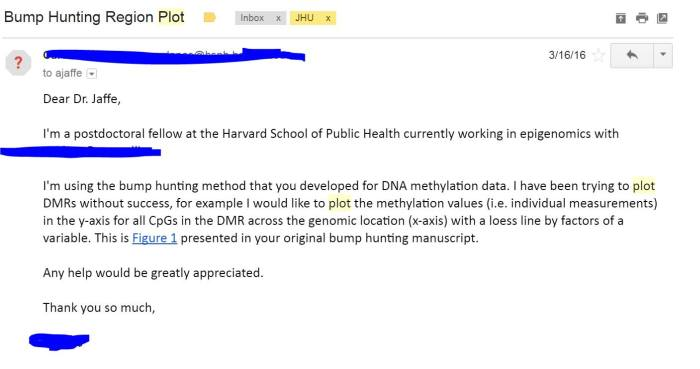
\includegraphics{media/code_request.jpg}
\caption{The paper came out January 2012 with code made in 2011}
\end{figure}

\end{frame}

\begin{frame}{Commenting in Scripts}
\protect\hypertarget{commenting-in-scripts-2}{}

\begin{figure}
\centering
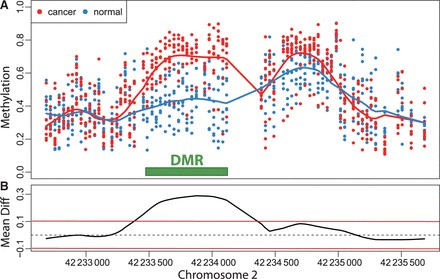
\includegraphics{media/dyr238f1.jpg}
\caption{This was the figure\ldots{}}
\end{figure}

\end{frame}

\begin{frame}{Commenting in Scripts}
\protect\hypertarget{commenting-in-scripts-3}{}

\begin{figure}
\centering
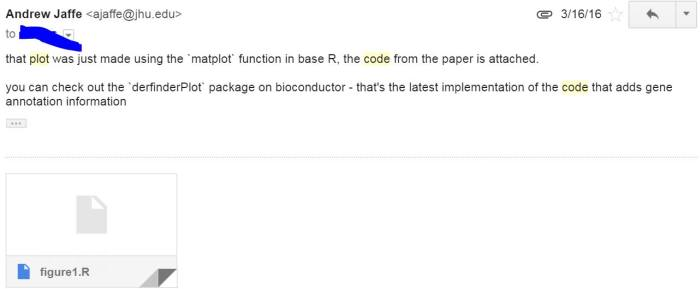
\includegraphics{media/code_fu.jpg}
\caption{After some digging, I found the code}
\end{figure}

\end{frame}

\begin{frame}[fragile]{Commenting in Scripts}
\protect\hypertarget{commenting-in-scripts-4}{}

Add a comment header to your script from today:\texttt{\#} is the
comment symbol

\begin{Shaded}
\begin{Highlighting}[]
\CommentTok{#################}
\CommentTok{# Title: Demo R Script}
\CommentTok{# Author: Andrew Jaffe}
\CommentTok{# Date: 7/13/2020}
\CommentTok{# Purpose: Demonstrate comments in R}
\CommentTok{###################}
 
\CommentTok{# nothing to its right is evaluated}

\CommentTok{# this # is still a comment}
\CommentTok{### you can use many #'s as you want}

\CommentTok{# sometimes you have a really long comment,}
\CommentTok{#    like explaining what you are doing }
\CommentTok{#    for a step in analysis. }
\CommentTok{# Take it to another line}
\end{Highlighting}
\end{Shaded}

\end{frame}

\begin{frame}[fragile]{R variables}
\protect\hypertarget{r-variables}{}

\begin{itemize}
\tightlist
\item
  You can create variables from within the R environment and from files
  on your computer
\item
  R uses ``='' or ``\textless-'' to assign values to a variable name
\item
  Variable names are case-sensitive, i.e.~X and x are different
\end{itemize}

\begin{Shaded}
\begin{Highlighting}[]
\NormalTok{x =}\StringTok{ }\DecValTok{2} \CommentTok{# Same as: x <- 2}
\NormalTok{x}
\end{Highlighting}
\end{Shaded}

\begin{verbatim}
[1] 2
\end{verbatim}

\begin{Shaded}
\begin{Highlighting}[]
\NormalTok{x }\OperatorTok{*}\StringTok{ }\DecValTok{4}
\end{Highlighting}
\end{Shaded}

\begin{verbatim}
[1] 8
\end{verbatim}

\begin{Shaded}
\begin{Highlighting}[]
\NormalTok{x }\OperatorTok{+}\StringTok{ }\DecValTok{2}
\end{Highlighting}
\end{Shaded}

\begin{verbatim}
[1] 4
\end{verbatim}

\end{frame}

\begin{frame}[fragile]{Help}
\protect\hypertarget{help}{}

For any function, you can write \texttt{?FUNCTION\_NAME}, or
\texttt{help("FUNCTION\_NAME")} to look at the help file:

\begin{Shaded}
\begin{Highlighting}[]
\NormalTok{?dir}
\KeywordTok{help}\NormalTok{(}\StringTok{"dir"}\NormalTok{)}
\end{Highlighting}
\end{Shaded}

\end{frame}

\begin{frame}[fragile]{Data Input}
\protect\hypertarget{data-input-4}{}

Initially-harder-but-gets-way-easier method: Utilizing functions in the
\texttt{readr} package called \texttt{read\_delim()} and
\texttt{read\_csv()} with code.

\end{frame}

\begin{frame}[fragile]{Data Input}
\protect\hypertarget{data-input-5}{}

So what is going on ``behind the scenes''?

\texttt{read\_delim()}: Read a delimited file into a data frame.

\begin{verbatim}
function (file, delim, quote = "\"", escape_backslash = FALSE, 
    escape_double = TRUE, col_names = TRUE, col_types = NULL, 
    locale = default_locale(), na = c("", "NA"), quoted_na = TRUE, 
    comment = "", trim_ws = FALSE, skip = 0, n_max = Inf, guess_max = min(1000, 
        n_max), progress = show_progress(), skip_empty_rows = TRUE) 
NULL
\end{verbatim}

\begin{verbatim}
# for example: read_delim("file.txt",delim="\t")
\end{verbatim}

\end{frame}

\begin{frame}{Data Input}
\protect\hypertarget{data-input-6}{}

\begin{itemize}
\tightlist
\item
  The filename is the path to your file, in quotes
\item
  The function will look in your ``working directory'' if no absolute
  file path is given
\item
  Note that the filename can also be a path to a file on a website
  (e.g.~`www.someurl.com/table1.txt')
\end{itemize}

\end{frame}

\begin{frame}[fragile]{Data Input}
\protect\hypertarget{data-input-7}{}

There is another convenient function for reading in CSV files, where the
delimiter is assumed to be a comma:

\begin{Shaded}
\begin{Highlighting}[]
\NormalTok{read_csv}
\end{Highlighting}
\end{Shaded}

\begin{verbatim}
function (file, col_names = TRUE, col_types = NULL, locale = default_locale(), 
    na = c("", "NA"), quoted_na = TRUE, quote = "\"", comment = "", 
    trim_ws = TRUE, skip = 0, n_max = Inf, guess_max = min(1000, 
        n_max), progress = show_progress(), skip_empty_rows = TRUE) 
{
    tokenizer <- tokenizer_csv(na = na, quoted_na = quoted_na, 
        quote = quote, comment = comment, trim_ws = trim_ws, 
        skip_empty_rows = skip_empty_rows)
    read_delimited(file, tokenizer, col_names = col_names, col_types = col_types, 
        locale = locale, skip = skip, skip_empty_rows = skip_empty_rows, 
        comment = comment, n_max = n_max, guess_max = guess_max, 
        progress = progress)
}
<bytecode: 0x000000001bfaa8d8>
<environment: namespace:readr>
\end{verbatim}

\end{frame}

\begin{frame}[fragile]{Data Input}
\protect\hypertarget{data-input-8}{}

\begin{itemize}
\tightlist
\item
  Here would be reading in the data from the command line, specifying
  the file path:
\end{itemize}

\begin{Shaded}
\begin{Highlighting}[]
\NormalTok{ufo =}\StringTok{ }\KeywordTok{read_csv}\NormalTok{(}\StringTok{"../data/ufo/ufo_data_complete.csv"}\NormalTok{)}
\end{Highlighting}
\end{Shaded}

\begin{verbatim}
Parsed with column specification:
cols(
  datetime = col_character(),
  city = col_character(),
  state = col_character(),
  country = col_character(),
  shape = col_character(),
  `duration (seconds)` = col_double(),
  `duration (hours/min)` = col_character(),
  comments = col_character(),
  `date posted` = col_character(),
  latitude = col_character(),
  longitude = col_double()
)
\end{verbatim}

\begin{verbatim}
Warning: 199 parsing failures.
 row col   expected     actual                                file
 877  -- 11 columns 12 columns '../data/ufo/ufo_data_complete.csv'
1712  -- 11 columns 12 columns '../data/ufo/ufo_data_complete.csv'
1814  -- 11 columns 12 columns '../data/ufo/ufo_data_complete.csv'
2857  -- 11 columns 12 columns '../data/ufo/ufo_data_complete.csv'
3733  -- 11 columns 12 columns '../data/ufo/ufo_data_complete.csv'
.... ... .......... .......... ...................................
See problems(...) for more details.
\end{verbatim}

The data is now successfully read into your R workspace, just like from
using the dropdown menu.

\end{frame}

\begin{frame}[fragile]{Data Input}
\protect\hypertarget{data-input-9}{}

The \texttt{read\_delim()} and related functions returns a ``tibble'' is
a \texttt{data.frame} with special printing, which is the primary data
format for most data cleaning and analyses.

\begin{Shaded}
\begin{Highlighting}[]
\KeywordTok{head}\NormalTok{(ufo)}
\end{Highlighting}
\end{Shaded}

\begin{verbatim}
# A tibble: 6 x 11
  datetime city  state country shape `duration (seco~ `duration (hour~ comments
  <chr>    <chr> <chr> <chr>   <chr>            <dbl> <chr>            <chr>   
1 10/10/1~ san ~ tx    us      cyli~             2700 45 minutes       This ev~
2 10/10/1~ lack~ tx    <NA>    light             7200 1-2 hrs          1949 La~
3 10/10/1~ ches~ <NA>  gb      circ~               20 20 seconds       Green/O~
4 10/10/1~ edna  tx    us      circ~               20 1/2 hour         My olde~
5 10/10/1~ kane~ hi    us      light              900 15 minutes       AS a Ma~
6 10/10/1~ bris~ tn    us      sphe~              300 5 minutes        My fath~
# ... with 3 more variables: `date posted` <chr>, latitude <chr>,
#   longitude <dbl>
\end{verbatim}

\begin{Shaded}
\begin{Highlighting}[]
\KeywordTok{class}\NormalTok{(ufo)}
\end{Highlighting}
\end{Shaded}

\begin{verbatim}
[1] "spec_tbl_df" "tbl_df"      "tbl"         "data.frame" 
\end{verbatim}

\end{frame}

\begin{frame}[fragile]{Data Input}
\protect\hypertarget{data-input-10}{}

\begin{Shaded}
\begin{Highlighting}[]
\NormalTok{ufo}
\end{Highlighting}
\end{Shaded}

\begin{verbatim}
# A tibble: 88,875 x 11
   datetime city  state country shape `duration (seco~ `duration (hour~ comments
   <chr>    <chr> <chr> <chr>   <chr>            <dbl> <chr>            <chr>   
 1 10/10/1~ san ~ tx    us      cyli~             2700 45 minutes       This ev~
 2 10/10/1~ lack~ tx    <NA>    light             7200 1-2 hrs          1949 La~
 3 10/10/1~ ches~ <NA>  gb      circ~               20 20 seconds       Green/O~
 4 10/10/1~ edna  tx    us      circ~               20 1/2 hour         My olde~
 5 10/10/1~ kane~ hi    us      light              900 15 minutes       AS a Ma~
 6 10/10/1~ bris~ tn    us      sphe~              300 5 minutes        My fath~
 7 10/10/1~ pena~ <NA>  gb      circ~              180 about 3 mins     penarth~
 8 10/10/1~ norw~ ct    us      disk              1200 20 minutes       A brigh~
 9 10/10/1~ pell~ al    us      disk               180 3  minutes       Strobe ~
10 10/10/1~ live~ fl    us      disk               120 several minutes  Saucer ~
# ... with 88,865 more rows, and 3 more variables: `date posted` <chr>,
#   latitude <chr>, longitude <dbl>
\end{verbatim}

\end{frame}

\begin{frame}[fragile]{Data Input}
\protect\hypertarget{data-input-11}{}

There are also data importing functions provided in base R (rather than
the \texttt{readr} package), like \texttt{read.delim} and
\texttt{read.csv}.

These functions have slightly different syntax for reading in data, like
\texttt{header} and \texttt{as.is}.

However, while many online resources use the base R tools, recent
versions of RStudio switched to use these new \texttt{readr} data import
tools, so we will use them in the class for slides. They are also up to
two times faster for reading in large datasets, and have a progress bar
which is nice.

\end{frame}

\begin{frame}[fragile]{Data Input - Excel}
\protect\hypertarget{data-input---excel}{}

Many data analysts collaborate with researchers who use Excel to enter
and curate their data. Often times, this is the input data for an
analysis. You therefore have two options for getting this data into R:

\begin{itemize}
\tightlist
\item
  Saving the Excel sheet as a .csv file, and using \texttt{read.csv()}
\item
  Using an add-on package, like \texttt{readxl}
\end{itemize}

For single worksheet .xlsx files, I often just save the spreadsheet as a
.csv file (because I often have to strip off additional summary data
from the columns)

For an .xlsx file with multiple well-formated worksheets, I use the
\texttt{readxl}package for reading in the data.

\end{frame}

\begin{frame}{Data Input - Other Software}
\protect\hypertarget{data-input---other-software}{}

\begin{itemize}
\tightlist
\item
  \textbf{haven} package
  (\url{https://cran.r-project.org/web/packages/haven/index.html}) reads
  in SAS, SPSS, Stata formats
\item
  \textbf{sas7bdat} reads .sas7bdat files
\item
  \textbf{foreign} package - can read all the formats as \textbf{haven}.
  Around longer (aka more testing), but not as maintained (bad for
  future).
\end{itemize}

\end{frame}

\begin{frame}[fragile]{Common new user mistakes we have seen}
\protect\hypertarget{common-new-user-mistakes-we-have-seen}{}

\begin{enumerate}
\tightlist
\item
  \textbf{Working directory problems: trying to read files that R
  ``can't find''}

  \begin{itemize}
  \tightlist
  \item
    RStudio can help, and so do RStudio Projects
  \item
    discuss in this Data Input/Output lecture
  \end{itemize}
\item
  Lack of comments in code
\item
  Typos (R is \textbf{case sensitive}, \texttt{x} and \texttt{X} are
  different)

  \begin{itemize}
  \tightlist
  \item
    RStudio helps with ``tab completion''
  \item
    discussed throughout
  \end{itemize}
\item
  Data type problems (is that a string or a number?)
\item
  Open ended quotes, parentheses, and brackets\\
\item
  Different versions of software
\end{enumerate}

\end{frame}

\begin{frame}[fragile]{Working Directories}
\protect\hypertarget{working-directories}{}

\begin{itemize}
\tightlist
\item
  R ``looks'' for files on your computer (or cloud) relative to the
  ``working'' directory
\item
  Many people recommend not setting a directory in the scripts

  \begin{itemize}
  \tightlist
  \item
    assume you're in the directory the script is in
  \item
    If you open an R file with a new RStudio session, it does this for
    you.
  \end{itemize}
\item
  If you do set a working directory, do it at the beginning of your
  script.
\item
  Example of getting and setting the working directory:
\end{itemize}

\begin{Shaded}
\begin{Highlighting}[]
\CommentTok{## get the working directory}
\KeywordTok{getwd}\NormalTok{()}
\KeywordTok{setwd}\NormalTok{(}\StringTok{"~/Lectures"}\NormalTok{) }
\end{Highlighting}
\end{Shaded}

\end{frame}

\end{document}
